\documentclass[10pt,a4paper]{article}
\usepackage[utf8]{inputenc}
\usepackage{amsmath}
\usepackage{amsfonts}
\usepackage{amssymb}
\usepackage{graphicx}
\usepackage{listings}
\author{Maria Coto-Sarmiento}
\title{Final project Summer School Data Driven, Pisa, 2016}

\begin{document}

\maketitle

\section{Introduction}


\subsection{Dataset}

We analized a dataset with amphorae from different places in order to understand the evolution of the amphorae made in different pottery workshops. Our dataset was collected from the project \emph{Roman Amphorae: a digital recourse} within Archaeology data service at University of Southampton (fig.\ref{picwebarch})

\begin{figure}[hdp]
	\centering
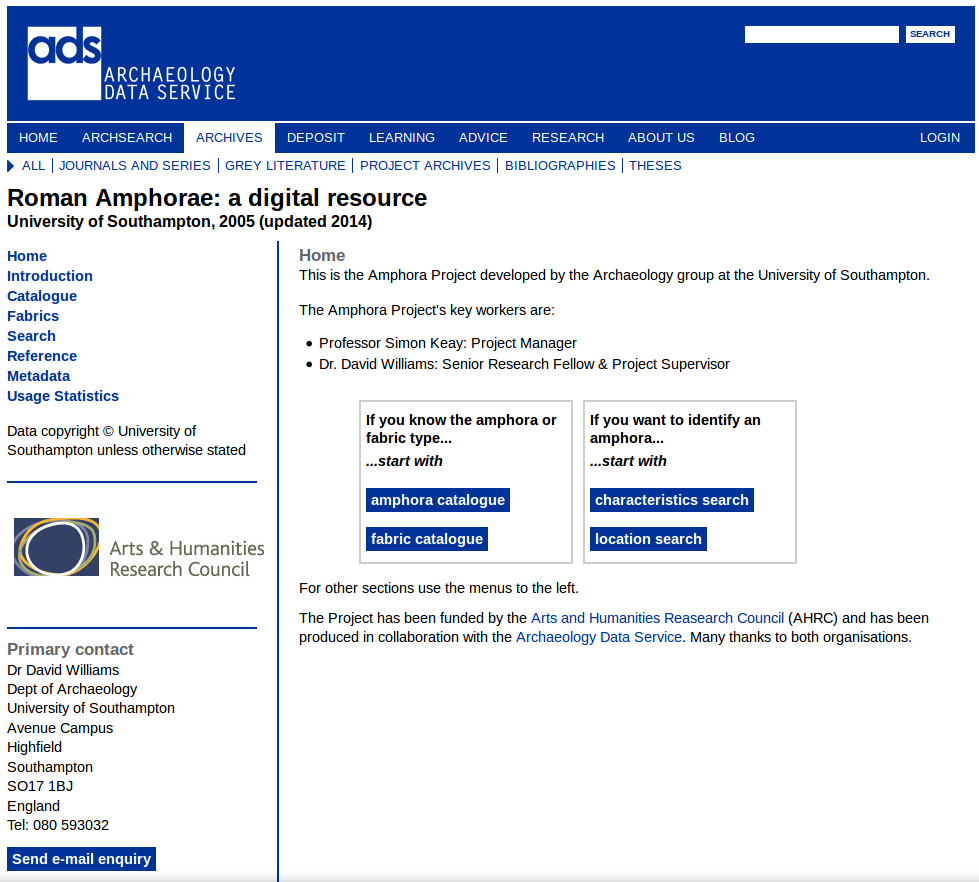
\includegraphics[scale=0.30]{picture1.png}
\label{picwebarch}
\caption{Webpage Roman Amphorae: a digital resource (Archaeology Data Service)}
\end{figure} 

This database is a catalogue of around 375 amphorae of different types and divided in different places and chronology during the Roman Empire. It was taken some characteristics on the dataset as the different parts of the shape of amphorae. 

Our dataset was divided in 24 columns:

\begin{itemize}
\item[-] \textbf{ID}: number of identification

\item[-] \textbf{Name}: type of amphorae 

\item[-] \textbf{Rim type}: divided into triangular (the rim has two straight, angled sides, resembling two partial sides of a triangle), everted (the rim becomes gently wider towards the top), collar (the rim is noticeably thickened in the form of a collar around the neck of the amphora), beaded (the rim has a simple rounded lip), rounded (the rim is gently rounded), flaring (the rim flares out sharply, in a more pronounced manner than an everted rim) and pulley wheel (this distinctive rim resembles a pulley-wheel). 

\item[-] \textbf{Shoulder type}: divided into rounded (the shoulder is noticeably present, usually supporting the handles, but there is no ridge), carinated (the shoulder displays distinct carination: a ridge where the shoulder meets the body of the amphora) and none/smooth (there is no shoulder: the body of the amphora is uninterrupted).

\item[-] \textbf{Handle profile}: divided into ear-shaped (these handles are similar to the 'curved' variety, but are more reminiscent of the shape of a human ear), bowed (the handles form a broad, curving sweep away from the body and neck of the amphora. They are generally longer than the 'curved' handles), curved (the handles gently curve from the neck to shoulder), peaked (the distinctive profile of these handles rises to a peak, often above the rim of the amphora. They are especially characteristic of the Rhodian type), ring (These handles are generally smaller than the 'curved' handles, forming a small semi-circular profile), short vertical (these handles travel upwards vertically from the shoulder, but only a short distance before turning inwards to the neck), arched(the handles form high arches, without coming to a point), long vertical(these handles generally appear on long-necked amphorae, attaching near the top of the neck progressing vertically downwards to the shoulder).

\item[-] \textbf{Handle section}: divided into ovoid/elliptical (the handle appears to be ovoid or elliptical in section), ridged (the handle has one or more ridges running down it), grooved (the handle is circular, or nearly circular, in section), round (the handle is circular, or nearly circular, in section), bifid (this is a distinctive feature of the Dressel 2-4 type. The handle is formed into two rods, appearing as a figure-8 in section).

\item[-] \textbf{Neck type}: divided into short/narrow (the neck is disproportionately short and/or narrow relative to the size of the amphora), cylindrical (the neck is cylinder-shaped), conical (the neck is cone-shaped - it tapers upwards), hourgrass (the neck takes the form of an hourglass, narrowing at its mid-point), none (there is no distinct neck: the body of the amphora progresses smoothly upwards to the rim) and broad (the neck tends to be wide)

\item[-] \textbf{Body type}: divided into cylindrical (the body of the amphora is cylinder-shaped, displaying little curvature), tapered (the body tapers downwards: it is wider at the top), globular (the body is wide, round and bag-shaped or globular), ovoid (the body is ovoid or elliptical in profile), piriform (the body is pear-shaped: it is wider towards the bottom of the amphora), narrow (the body is disproportionately narrow compared with the height of the amphora)

\item[-] \textbf{Base type} divided into short hollow (the base is short and hollow), spike/tapered (there is a solid spike at the base of the amphora), knobbed (there is small knob at the base of the amphora), ringed (the base has a foot ring), button (there is a noticeable button-shape at the base of the amphora), flat (the base has been flattened so the amphora will stand unsupported), long hollow (the base and foot are long and hollow), pointed (the base comes to a point), rounded basal point (the base extends into a small, pronounced point not as long as a spike)

\item[-] \textbf{Capacity}: capacity of the amphorae

\item[-] \textbf{Height min}: minimum height

\item[-] \textbf{Height max}: maximum height

\item[-] \textbf{Width min}: minimum width

\item[-] \textbf{Rim diameter min}: minimum rim diameter

\item[-] \textbf{Rim diameter max}: maximum rim diameter

\item[-] \textbf{Manufacture}: workshops where amphorae come from 

\end{itemize}


\section{Objetives}

The aim of this project can be divided in different objectives: 

\begin{itemize}
\item[-] A simple exploration of our dataset. We focus our dataset to seek the kind of information that we are going to work. So we need to fit our database to each exercises. 
\item[-] In particular, we want to explore the differences among workshops from different places. We can detect measurable differences in the amphorae production over time as the result of different pattern of production. 
\item[-] The exercises will be different adapted to each section. Specifically, we want to focus this project in \textit{Dressel} production. For that, we want to use the amphorae measurement to analyze the production differences. 
\end{itemize}


\section{MySQL}

We used phpMyAdmin, a free software tool to handle the administration of MySQL  with Linux and perform our data (fig.\ref{myphp})

\begin{figure}[hdp]
	\centering
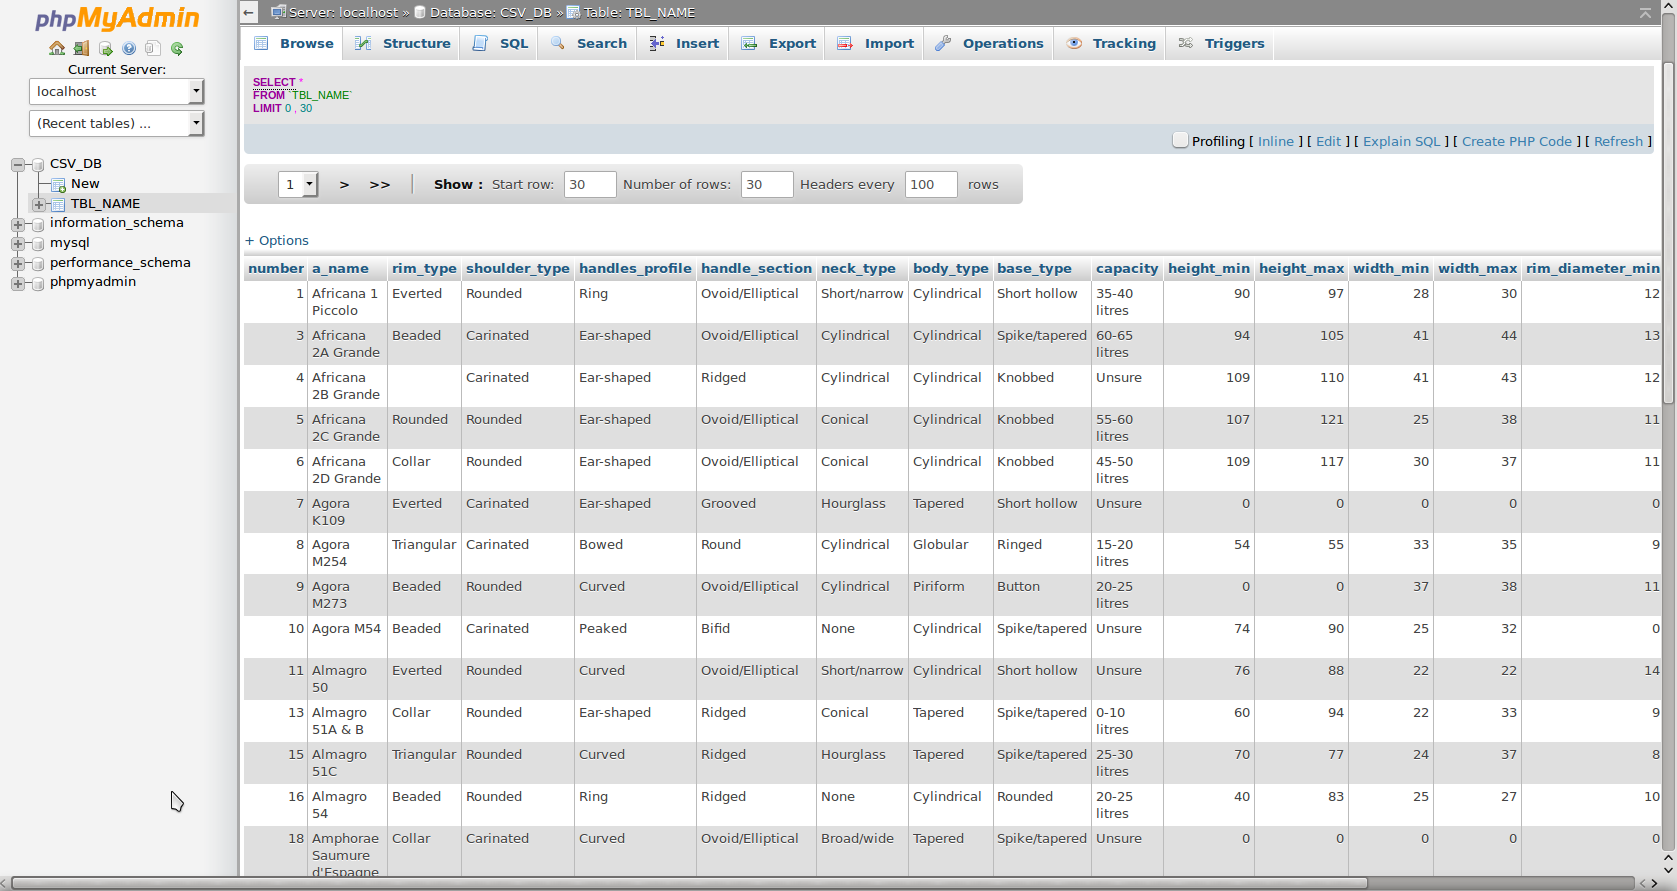
\includegraphics[scale=0.25]{picture2.png}
\label{myphp}
\caption{phpMyAdmin program with the database}
\end{figure} 

\subsection{MySQL exercises}

We perform some exercises with mySQL and query the dataset. 

\subsubsection{Exercise 1}

We want to know how many rim shapes are "everted". For that, we used the following code

\begin{verbatim}
SELECT *
FROM `TBL_NAME`
WHERE `rim_type` = "everted"
LIMIT 0 , 30
\end{verbatim}


We select all from our dataset but we want specifically to select from the column rim type the types which are everted. We also specify a limit by 30 (fig. \ref{query1})

\begin{figure}[hdp]
     \centering
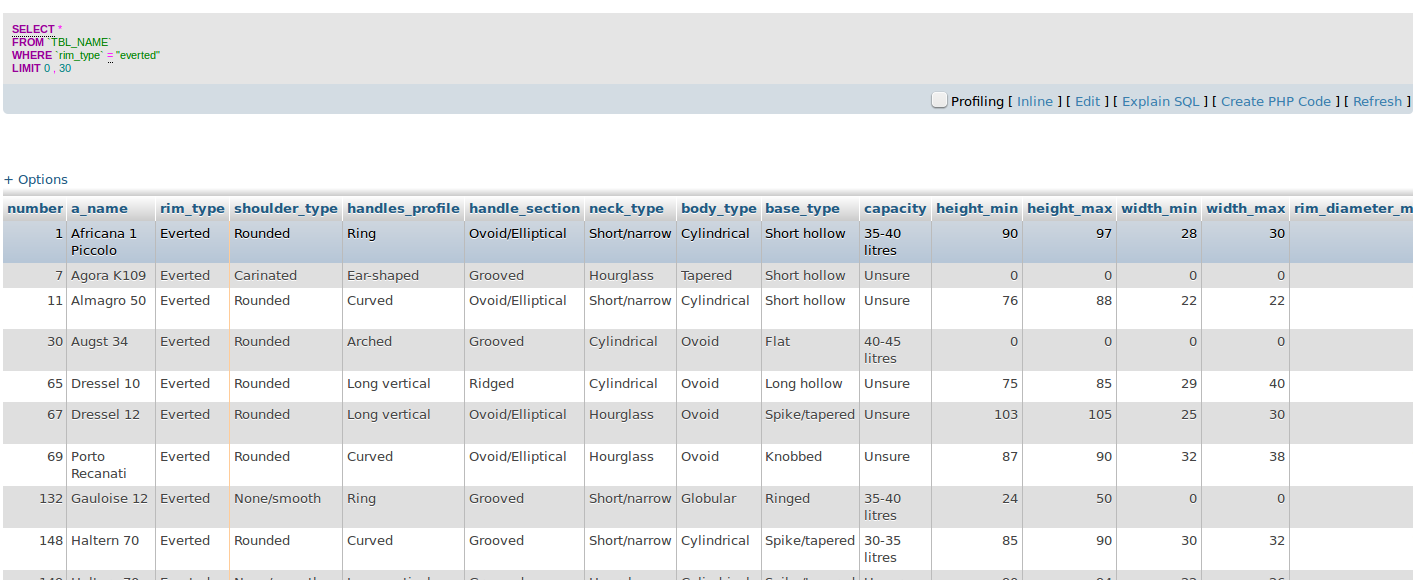
\includegraphics[scale=0.30]{output_query1.png}
\label{query1}
\caption{query selecting "everted"}
\end{figure} 



\subsubsection{Exercise 2}

We want to know how many amphorae have a cylindrical body type. We use the following code

\begin{verbatim}
SELECT `a_name`
FROM `TBL_NAME`
WHERE `body_type` = "cylindrical"
\end{verbatim}

We select the column $a\_name$ from the general table on the dataset. We also select from the body type column which amphorae are cylindrical (fig. \ref{query2}). 

\begin{figure}[hdp]
\centering
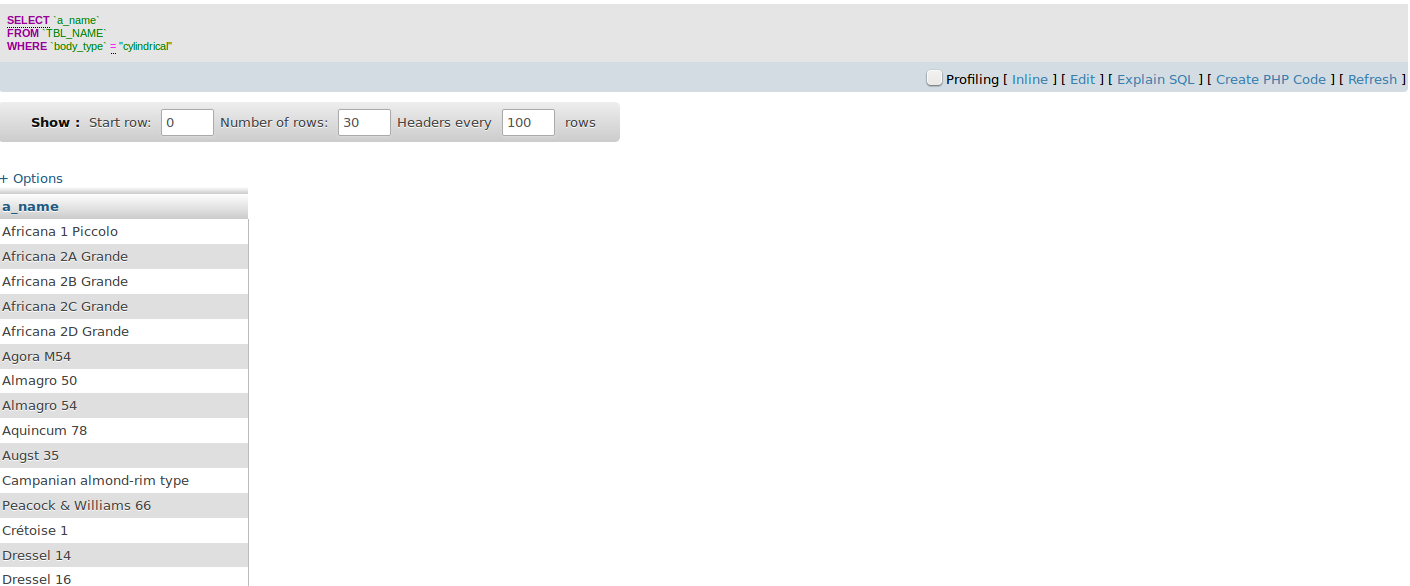
\includegraphics[scale=0.30]{query2.png}
\label{query2}
\caption{query selecting cylindrical column}
\end{figure} 


\subsubsection{Exercise 3}

We want to know which amphorae have the largest diameter. We use the following code

\begin{verbatim}
SELECT `a_name` , `rim_diameter_max`
FROM `TBL_NAME`
ORDER BY `rim_diameter_max` DESC
LIMIT 100 
\end{verbatim}

We select the columns and ORDER BY in order to know which diameter is the largest. We can choose between ASC (ascending order) or DESC (descending order) (fig. \ref{query3})

\begin{figure}[hdp]
\centering
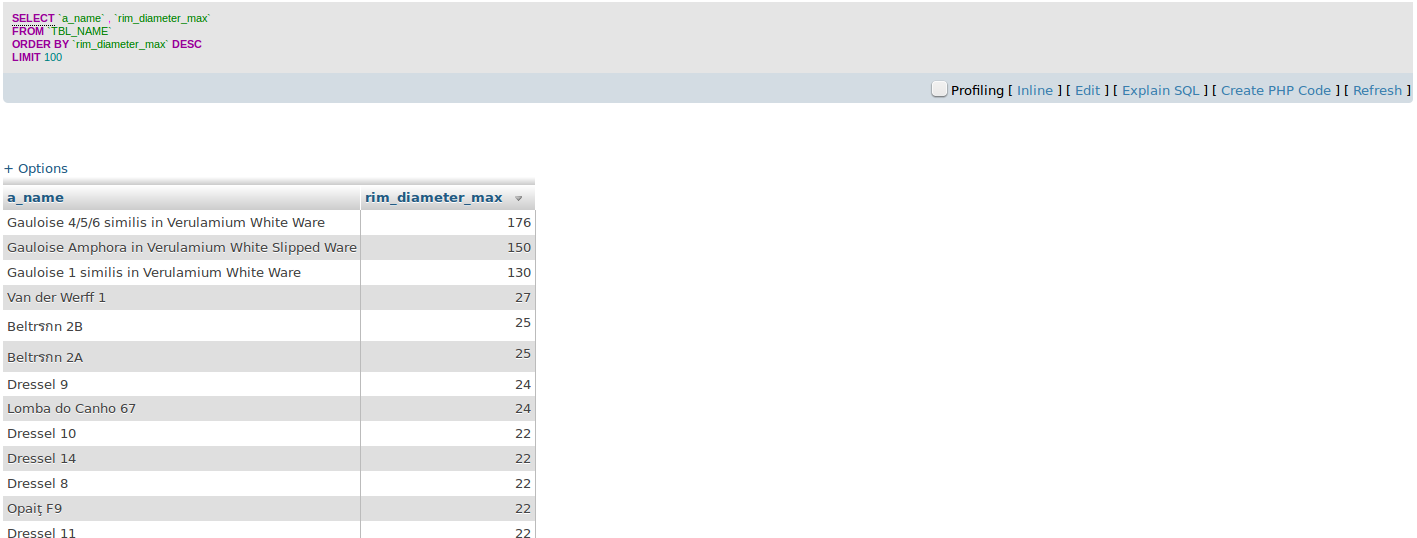
\includegraphics[scale=0.30]{query3.png}
\label{query3}
\caption{query selecting two columns ordered by maximum diameter}
\end{figure} 

\subsubsection{Exercise 4}

We want to know which amphorae have cylindrical body type and carinated shoulder type with a limit of 100. We also want to order by alphabetical name of amphorae. 

\begin{verbatim}
SELECT `a_name` , `shoulder_type` , `body_type`
FROM `TBL_NAME`
WHERE `shoulder_type` = "carinated"
AND `body_type` = "cylindrical"
ORDER BY `a_name`
LIMIT 0 , 100
\end{verbatim}

We select three columns from the original table and we specifically choose body type, shoulder type and $a\_name$ ordered by names of amphorae (fig. \ref{query4})

\begin{figure}[hdp]
\centering
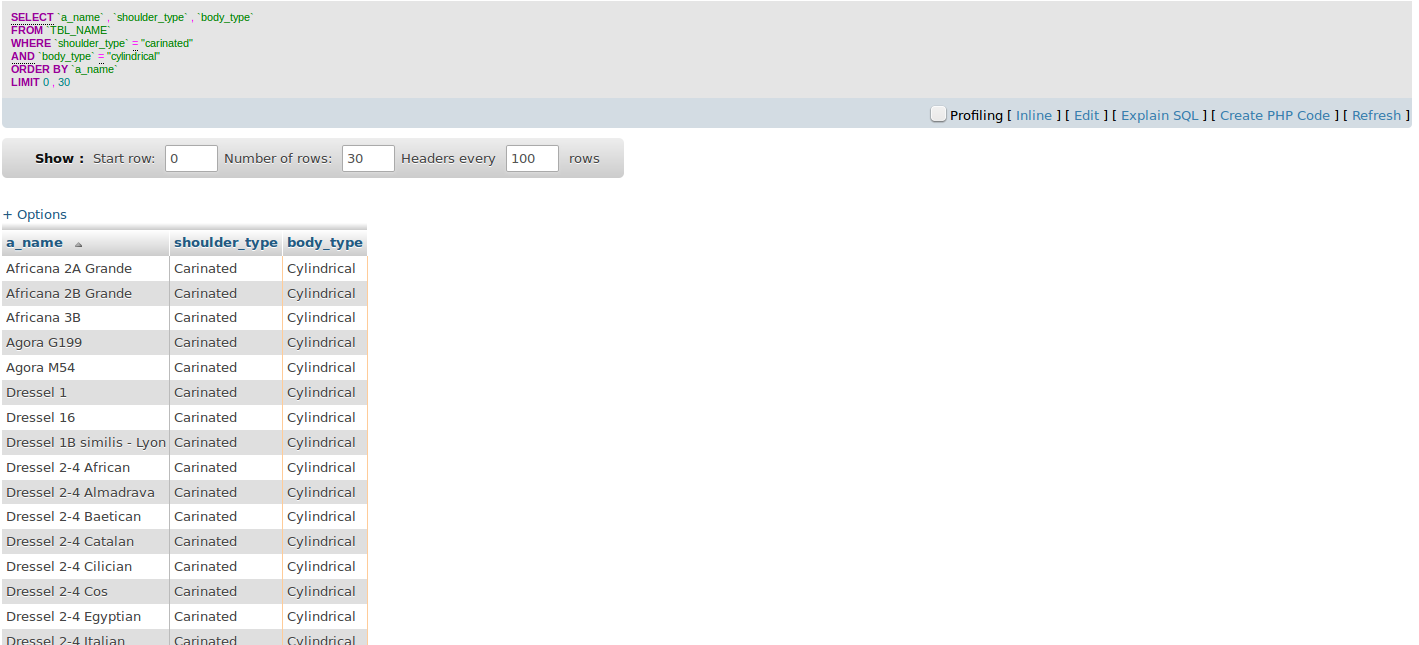
\includegraphics[scale=0.30]{query4.png}
\label{query4}
\caption{query selecting shoulder type, body type and type of amphorae}
\end{figure} 


\subsection{Querying the data}

For our database, we want to select the Dressel types and its maximum and minimum diameters. We are going to analyze the differences between diameters and whether are related with the workshops of each type of amphorae. 

\begin{verbatim}
SELECT `a_name` , `rim_diameter_min` , `rim_diameter_max` , `manufacture`
FROM `TBL_NAME`
WHERE `a_name` LIKE "%Dressel%"
ORDER BY `a_name` ASC
LIMIT 0 , 100
\end{verbatim}

To do that, we select the type of amphorae, maximum and minimum diameter and manufacture columns from the general table. We only want to select Dressel types so we use LIKE \$Dressel\$ to select only the Dressel types in the database. The database will be ordered by names with the command ORDER BY and with ascending order. The limit must be until 100 to select all the amphorae as possible (fig. \ref{query5})

\begin{figure}[hdp]
\centering
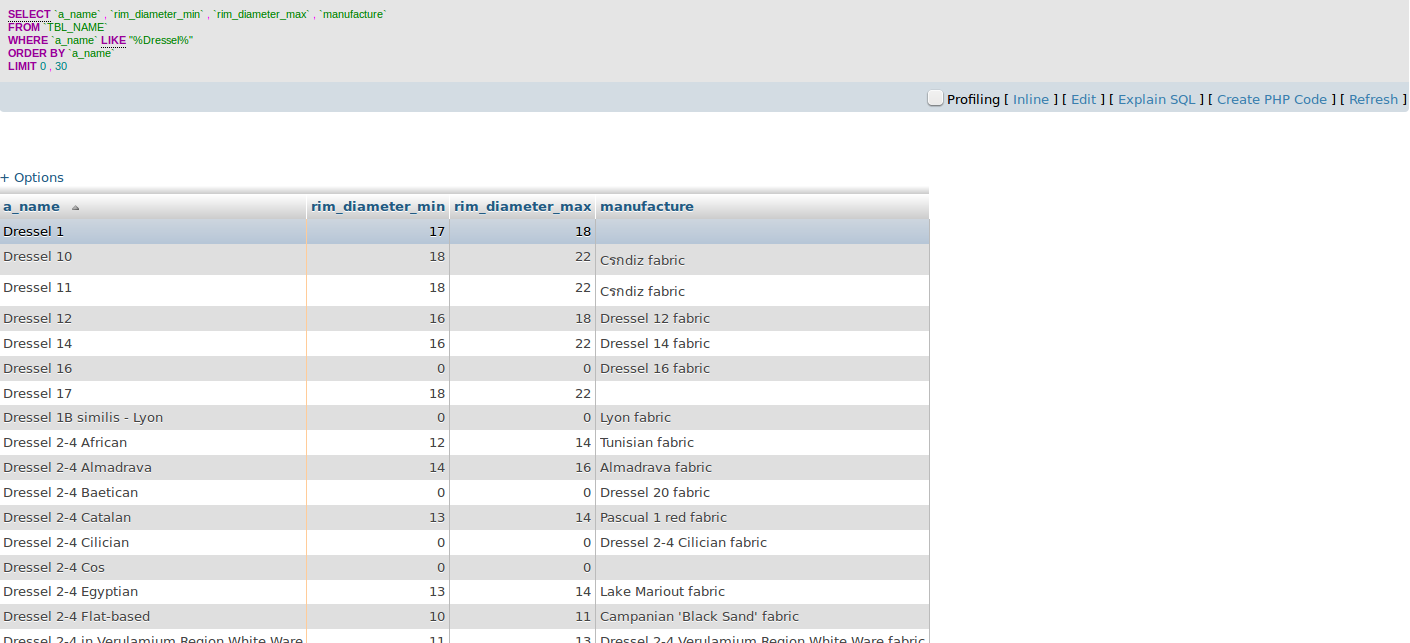
\includegraphics[scale=0.30]{query5.png}
\label{query5}
\caption{Database selected with Dressel amphorae}
\end{figure} 

\section{R programming language exercises}

We explored the database produced by MySQL with R program. Thus, we have used R programming language in the command line in order to analyse the data. However, R Studio was not used in this exercise. 

\subsection{Calculate the mean with R program}

We want to calculate the mean of maximum and minimum diameter of the amphorae to know the differences of the diameters. ALARGAR

We use the following code with R to calculate the mean maximum and minimum diameter

\begin{verbatim}
project= project$rim_diameter_max
mean (project)
[1] 13.1
\end{verbatim}

\begin{verbatim}
project= project$rim_diameter_min
mean (project)
[1] 10.95
\end{verbatim}

We also wanted to calculate the frequency of maximum diameter in our database to know which measurement of diameter is more frequent in our database. 

We perform with the following code

\begin{verbatim}
hist(project$rim_diameter_max, border= "white", col= "black", 
main= "Frecuency of maximum diameter")
\end{verbatim}

We create an histogram with the frequency of the maximum diameter. We perform the histogram with black color and white borders. We put a title with the command "main" (fig. \ref{histomax}).

\begin{figure}[hdp]
\centering
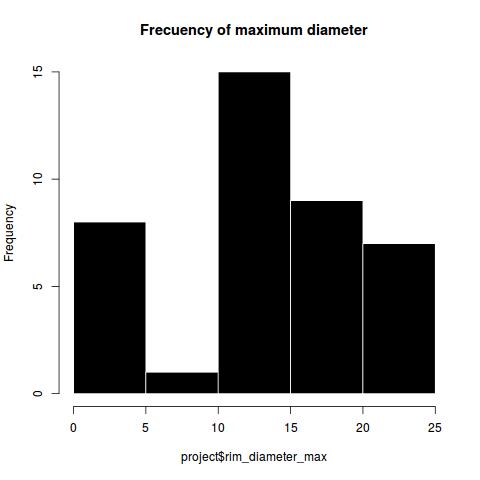
\includegraphics[scale=0.40]{histomax.png}
\label{histomax}
\caption{Histogram with the frequency of maximum diameter}
\end{figure} 

Likewise, the same code was also used to calculate the frequency of minimum diameter as well. 

\begin{verbatim}

boxplot(project$rim_diameter_min, main= "Frecuency of minimum diameter")

\end{verbatim}

We use the boxplot graphic to visualize the frequency of minimum diameter (fig. \ref{boxmin})

\begin{figure}[hdp]
\centering
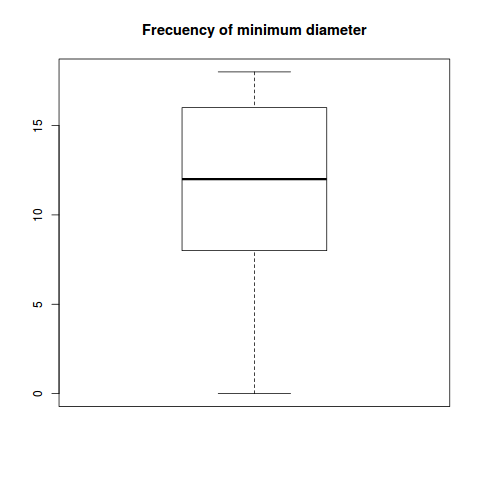
\includegraphics[scale=0.50]{boxplotmin.png}
\label{boxmin}
\caption{Boxplot with the frequency of minimum diameter}
\end{figure} 

\subsection{Exercises using different graphing packages/libraries} 


\subsubsection{qplot}

We used the graphing package qplot to plot the results of diameter with the pottery workshops to know if there are differences among them (fig. \ref{qplot}). We also performed the color scale to differentiate the pottery workshops 

\begin{verbatim}
qplot(x= rim_diameter_max, y= rim_diameter_min, data= project, 
main= "Frecuency", color= manufacture) 
\end{verbatim}

\begin{figure}[hdp]
\centering
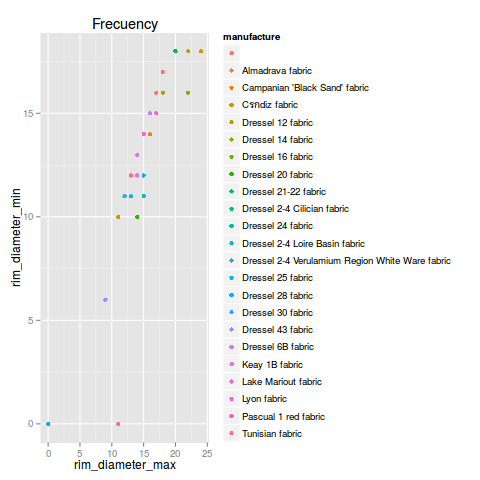
\includegraphics[scale=0.50]{qplotminmax.png}
\label{qplot}
\caption{Using qplot graphing package}
\end{figure}



\subsubsection{ggplot2}

We wanted to see the diameter differences among pottery workshops ("manufacture") and type of amphorae. 

We had to install the package ggplot2 before performing the data to use it as graphing library 

\begin{verbatim}
install.package ("ggplot2")
library (gglot2)
\end{verbatim}

Then, we use the following code: 

We are going to select different types of pottery workshops such as C\'adiz fabric, Tunisian fabric, Dressel 20 fabric and Dressel 24 fabric because we want to know the differences in the production

\begin{verbatim}
myData= subset(project, manufacture  %in% c("Cdiz fabric", 
"Tunisian fabric", "Dressel 20 fabric", "Dressel 24 fabric"))

\end{verbatim}

We select from our database the type of amphorae and the pottery workshops ("manufacture") and we plot the results 

\begin{verbatim}
ggplot(myData, aes(x=rim_diameter_max, y=rim_diameter_min, colour= manufacture)) 
+ geom_point() + facet_wrap(~a_name)
\end{verbatim}

We divided the different amphorae types to see the differences among diameter related with the pottery workshops (manufacture in the picture fig. \ref{ggplotex})


\begin{figure}[hdp]
\centering
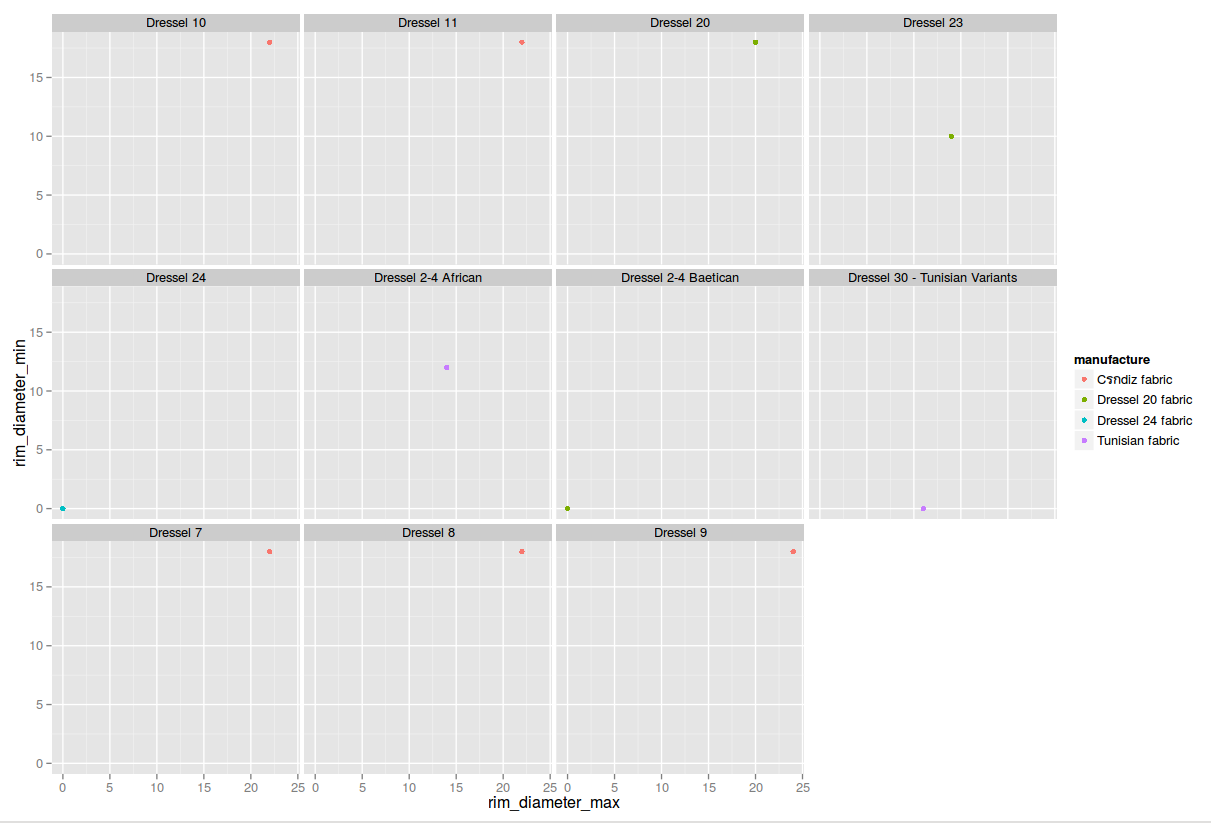
\includegraphics[scale=0.45]{ggplot2ex.png}
\label{ggplotex}
\caption{Using ggplot graphics}
\end{figure}


\section{Mapping the data. Ontological section}

\subsection{CIDOC-CRM exercises}

We want to develop the ontological process based on the pottery production. We used the following ontological entities from CIDOC-CRM, a semantic framework used in cultural heritage, to define our data (fig. \ref{sparex}). Then we represented our result in a graphic with the schema mapping. 

\begin{itemize}
\item[-] \textbf{E.55 Type} (because we have represented a pottery database)
\item[-] \textbf{E.57 Material} (represented by amphorae)
\item[-] \textbf{P.108 was produced by} (represented by potters)
\item[-] \textbf{E.12 Production} (pottery workshops)
\item[-] \textbf{P.31 Has modified by} (made and modified by potters)
\item[-] \textbf{P.14 Carry out by} (represented by potters and workshops)
\item[-] \textbf{E.24 Physical made man things} (represented by potters)
\item[-] \textbf{E.39 Actor} (represented by potters who make pottery)
\item[-] \textbf{E.53 Place} (represented by the production site)
\item[-] \textbf{P.53 has former or current location} (production site)
\end{itemize}


\begin{figure}[hdp]
\centering
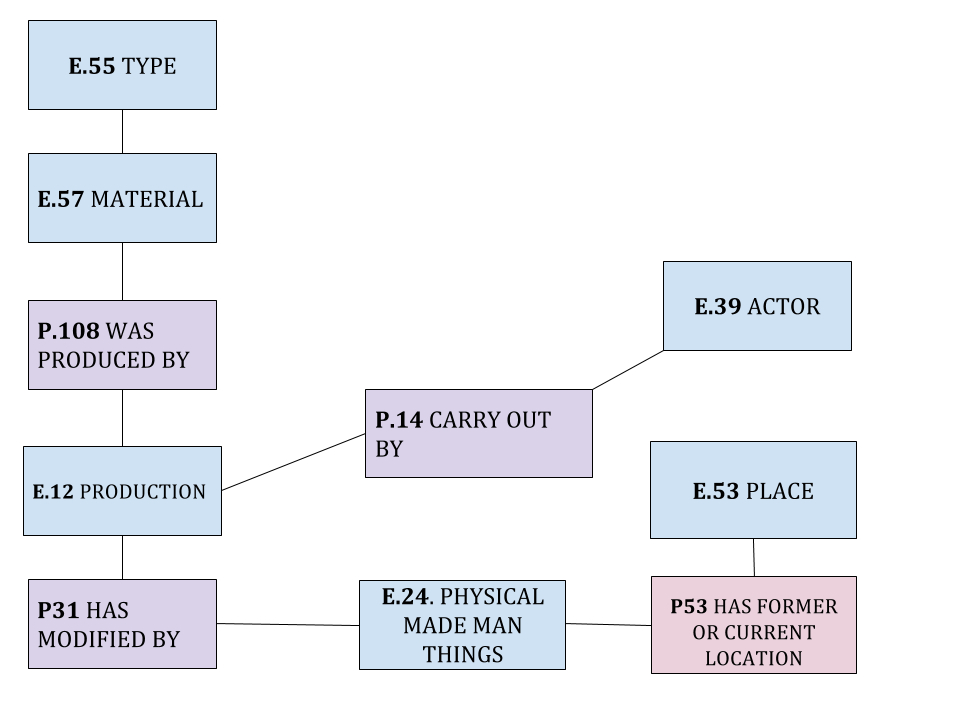
\includegraphics[scale=0.50]{sparex.png}
\label{sparex}
\caption{Mapping representing data with CIDOC-CRM}
\end{figure}


\section{Licenses and data}

We have selected for our data the licence created by Creative Common. In our case, we believe in the free distribution of open data so we chose the licence CC BY-SA. This kind of license allows to modify, develop and use the data, even with commercial purposes. This license also allows to use new creations under the identical terms and indicate if changes were made in our data. (fig. \ref{licence})

We think that it could be a good licence for our data because it allows to share our data for free. 

\begin{figure}[hdp]
\centering

\includegraphics[scale=0.15]{licence.png}
\label{licence}
\caption{Type of license CC BY-SA}
\end{figure}


\section{Analize data on QGIS}

\subsection{Performing the data with Open Refine}

We created a new dataset to transform with Open Refine and geolocalize the results with QGIS. We use the data from the pottery workshops of \emph{Baetica} (currently Andalusia), ancient province within Roman Empire. In particular, We collected in the database the workshops of amphorae of olive oil. This commerce was particularly important due to the high demand of olive oil in the Roman Empire. As result, a huge network of pottery workshops were created to satisfy this demand. 

As a first step, we perform our data with Open Refine

\begin{itemize}
\item[-] We open our data on Open Refine server
\item[-] We select the column where we want to edit. In the column, we select Edit Column and the option Add column by fetching URLs for the geolocalization
\item[-]We add in expression option the following code (fig. \ref{openrefine1}) 
\begin{verbatim}
"http://maps.google.com/maps/api/geocode/json?sensor=false&add
ress=" + escape(value, "url")
\end{verbatim}

\begin{figure}[hdp]
\centering
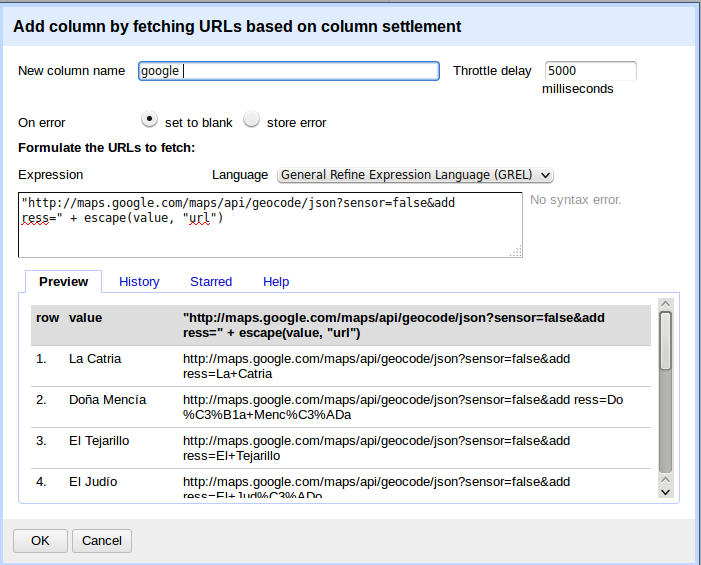
\includegraphics[scale=0.50]{openrefine1.png}
\label{openrefine1}
\caption{Add geolocalization on Open Refine}
\end{figure}

\item[-] When the file finishes loading,  we select Edit cells and Transform. We write the next code to transform in latitude and longitude (fig. \ref{openrefine2})
\begin{verbatim}
with(value.parseJson().results[0].geometry.location, pair, pair.lat +",
" + pair.lng)
\end{verbatim}

\begin{figure}[hdp]
\centering
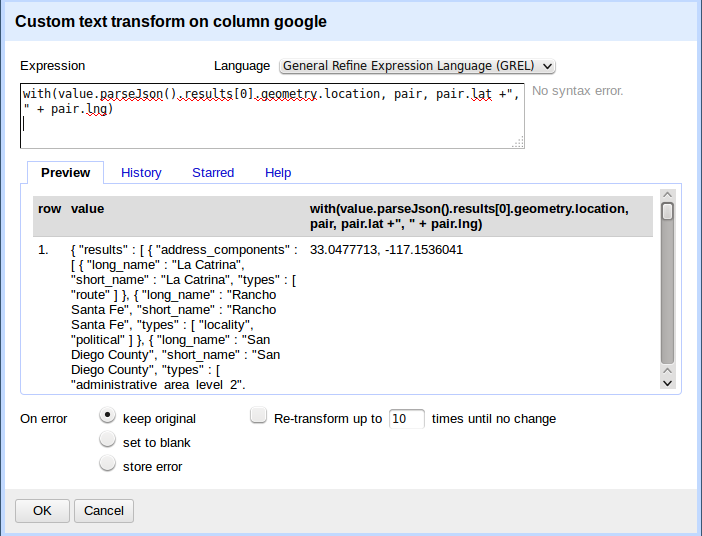
\includegraphics[scale=0.50]{openrefine2.png}
\label{openrefine2}
\caption{Transform the data in latitude and longitude}
\end{figure}
\item[-] We select edit column and the option Split into several column to separate into two different columns (fig. \ref{openrefine3})

\begin{figure}[hdp]
\centering
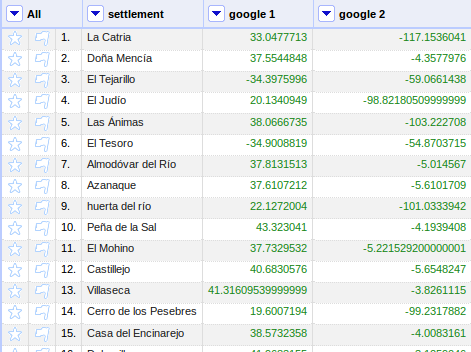
\includegraphics[scale=0.50]{openrefine3.png}
\label{openrefine3}
\caption{Transform the data in latitude and longitude}
\end{figure}

\item[-] We export the results as csv file 
\end{itemize}


\subsection{QGIS}

We use the database performed by Open Refine to produce a spatial visualization on QGIS. We had to modify our dataset because some pottery workshops did not detect real coordinates. These pottery workshops were deleted and we just include the pottery workshops correctly geolocalized. Ultimately, our data were performed with QGIS version 2.0.1 Dufour on Linux Mint. 
\\

We follow the steps below:
\begin{itemize}
\item[-] We choose in Layer option Add Delimiter Tex Layer to attach the csv file. You also can do it in the Toolbars on the left (fig. \ref{gismap2})
\begin{figure}[hdp]
\centering
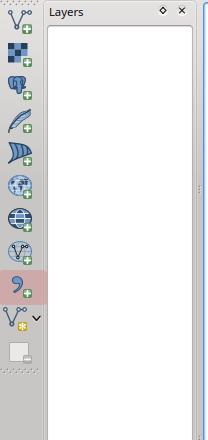
\includegraphics[scale=0.50]{gismap2.png}
\label{gismap2}
\caption{Option (in red) to attach the document file}
\end{figure}
\item[-] We attach the file that we want to use it and the format. In geometrical definition option we have to be sure for choosing the accurate latitude and longitude (fig. \ref{gismap3})

\begin{figure}[hdp]
\centering
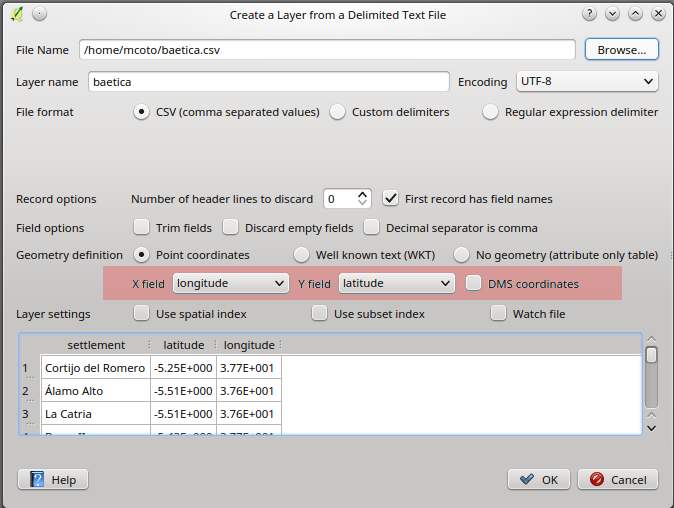
\includegraphics[scale=0.50]{gismap3.png}
\label{gismap3}
\caption{Option of geometry definition and coordinates}
\end{figure}

\item[-] We need to map our result. So we have to select Manage in the plugins option and install plugins and "get more" to install Open Layers. Open Layers is a plugin library to show and manipulate maps from different application on internet. In Linux, this API has to be installed thought Python. So we have to install first OpenLayer plugin on Python (fig. \ref{gismap4})

\begin{figure}[hdp]
\centering
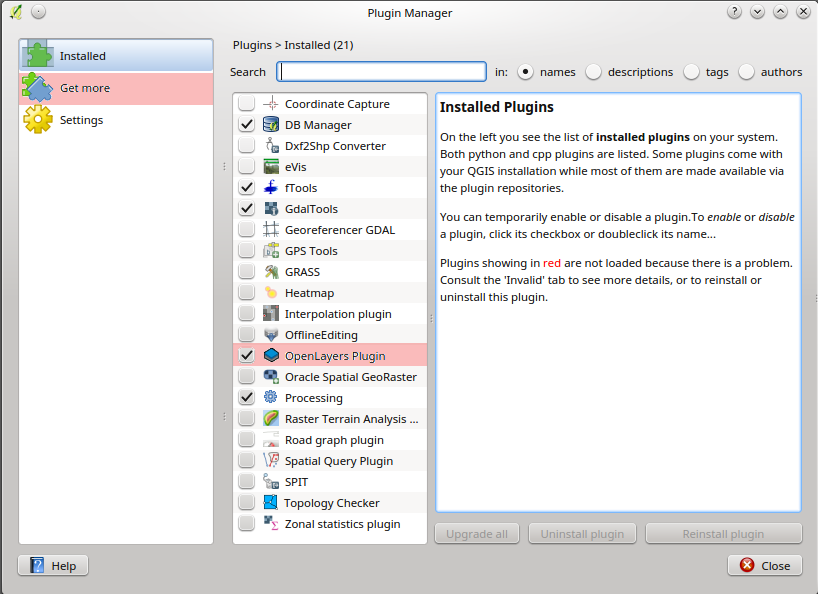
\includegraphics[scale=0.50]{gismap4.png}
\label{gismap4}
\caption{Install and select OpenLayers Plugin}
\end{figure}

\item[-] Once installed, we choose the most accurate map server to geolocalize our results. In our case, we chose Open Street Maps Layer. 
\item[-] We map the database. Our result we can see a homogeneous dispersion of the pottery workshops. This dispersion concur with necessity to build the workshops next to rivers in order to pick up clay from the rivers and make pottery artifacts.   (fig. \ref{gismap})

\begin{figure}[hdp]
  \centering
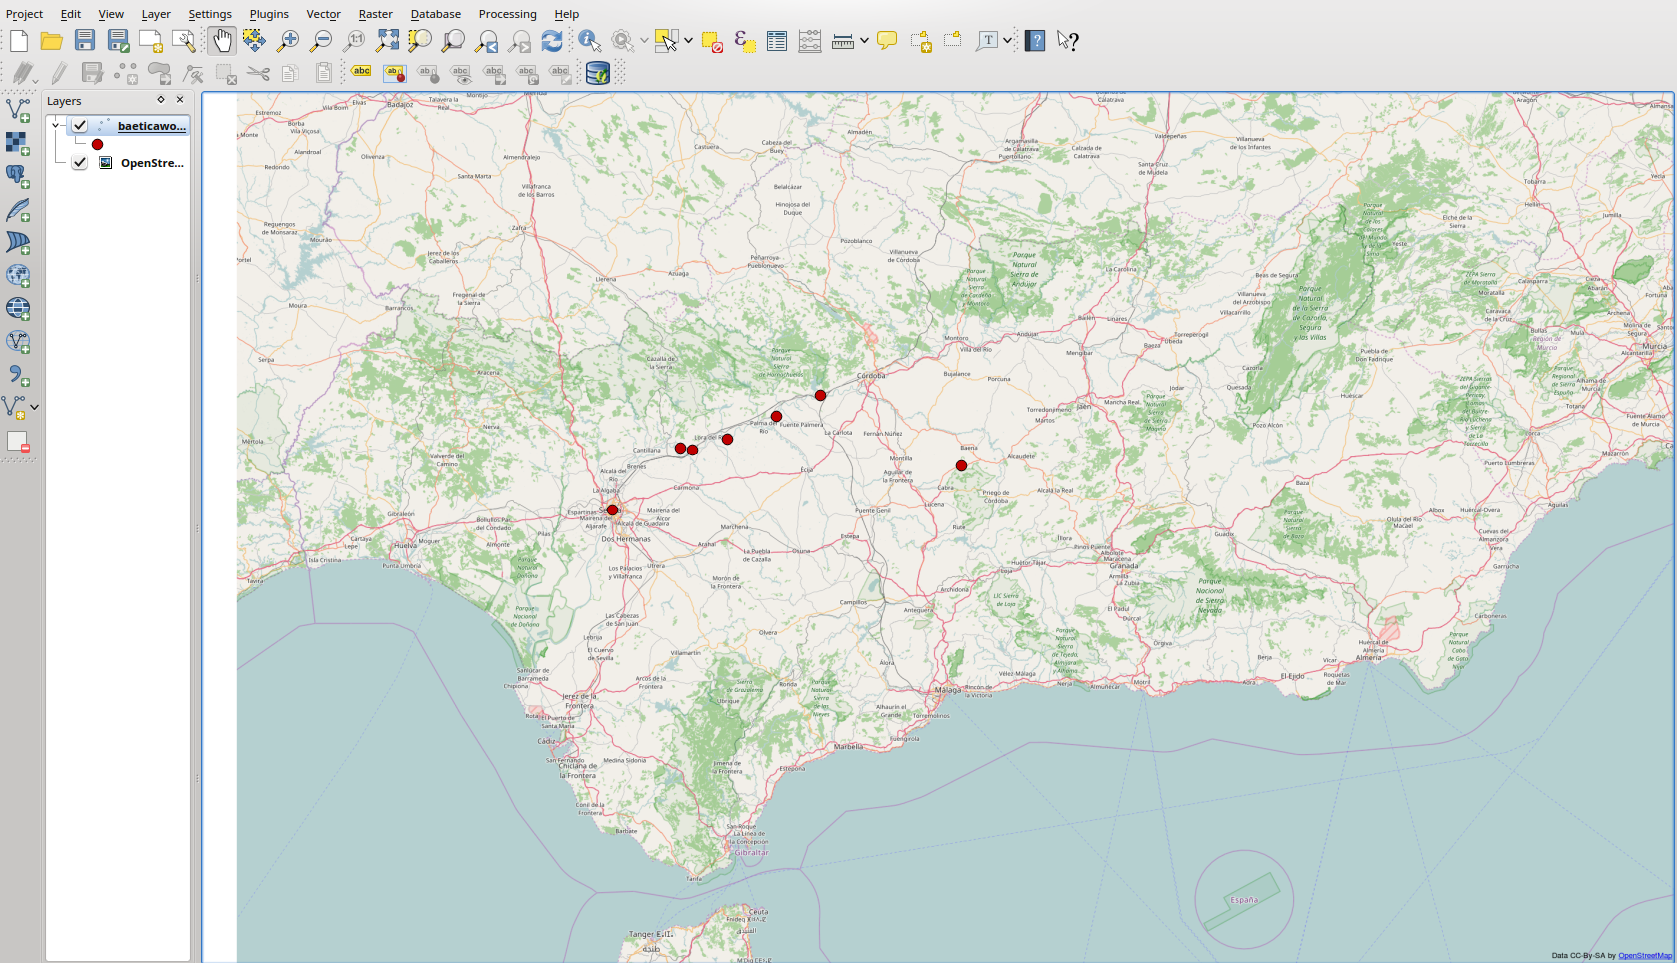
\includegraphics[scale=0.30]{gismap.png}
\label{gismap}
\caption{Mapping of the database}
\end{figure}

\end{itemize}

\subsection{Discussion and Conclusion}

It is a exploration of data so our results are not finished yet. 









































 



\end{document}